\section{Gradient-Norm Dynamics and Solver Order}
\label{sec:track-b}

The benchmark ablation found Forward Euler uniquely unable to reach $10^{-4}$
training loss within budget, with $28\times$ worse extrapolation MSE than
Tsit5 (Table~\ref{tab:solver-ablation}). The candidate mechanism tested here: a
first-order solver commits an $O(h^2)$ local error every step, accumulating to
an $O(h)$ global error, which could
inject measurably noisier gradients and destabilize Adam's moment estimates.

\begin{expectbox}
\expectrow{Question}{Does a lower-order solver's larger truncation error show up as measurably noisier gradients during training?}
\expectrow{Expected}{Gradient-norm noise should fall as solver order rises, correlating with the accuracy ranking already seen in the benchmark ablation.}
\expectrow{Observed}{No reliable correlation ($\rho=-0.088$, $p=0.87$); the ranking is non-monotone and its sign flips depending on an arbitrary warm-up cut. Refuted.}
\end{expectbox}

The noise measure is the standard deviation of epoch-to-epoch \emph{relative}
gradient change, scale-invariant by construction,
\begin{equation}
\eta = \operatorname{std}\big(\Delta\log_{10} g\big), \qquad
\Delta\log_{10} g_i = \log_{10} g_{i+1} - \log_{10} g_i,
\label{eq:noise-measure}
\end{equation}
compared against solver order $p$ by Spearman rank correlation rather than
the more familiar Pearson correlation. Pearson correlation measures how
linearly two quantities move together, which presumes solver order is a
quantity whose actual numeric spacing is meaningful -- that the jump from
order 1 to order 2 is comparable in size to the jump from order 4 to order
5. There is no reason to expect $\eta$ to depend on solver order that
linearly; the hypothesis under test is only that noise falls
\emph{monotonically} as order rises, which is exactly what Spearman
correlation measures, by comparing ranks rather than raw values. It also
handles the ties at $p=2$ (Heun, Midpoint) and $p=5$ (DOPRI5, Tsit5)
natively, where Pearson would need an arbitrary tie-breaking rule.

\begin{table}[!ht]
\centering
\small
\renewcommand{\arraystretch}{1.15}
\caption{Gradient-noise measure $\eta$ vs.\ solver order, six solvers, $n=6$.}
\label{tab:gradient-noise}
\begin{tabularx}{\textwidth}{@{}L{2.6cm} C{1.3cm} C{1.6cm} C{2.2cm} X@{}}
\toprule
\hdrrow \thh{Solver} & \thh{Order $p$} & \thh{Noise $\eta$} & \thh{Best training MSE} & \thh{Noise rank}\\
\midrule
Forward Euler & 1 & $0.2805$ & $1.377\times10^{-4}$ & 1 (noisiest)\\
Classical RK4 & 4 & $0.2726$ & $9.413\times10^{-5}$ & 2\\
Tsit5 & 5 & $0.2683$ & $8.833\times10^{-5}$ & 3\\
DOPRI5 & 5 & $0.2660$ & $9.283\times10^{-5}$ & 4\\
Midpoint RK2 & 2 & $0.2634$ & $8.857\times10^{-5}$ & 5\\
Heun RK2 & 2 & $0.2621$ & $8.315\times10^{-5}$ & 6\\
\bottomrule
\end{tabularx}
\end{table}

Spearman $\rho=-0.088$, $p=0.87$ ($n=6$). Three findings jointly refute the
hypothesis: the effect size is a 7\% spread across all six solvers; the
ranking is non-monotone (RK4, order 4, is the second-noisiest solver); and the
sign of $\rho$ flips across warm-up cuts ($-0.088\to-0.441\to+0.706$ as the
first 0, 2000, 5000 epochs are dropped); no cut reaches significance
($p\ge0.12$), and the direction of any relationship depends on an arbitrary
analyst choice.

\begin{figure}[htbp]
\centering
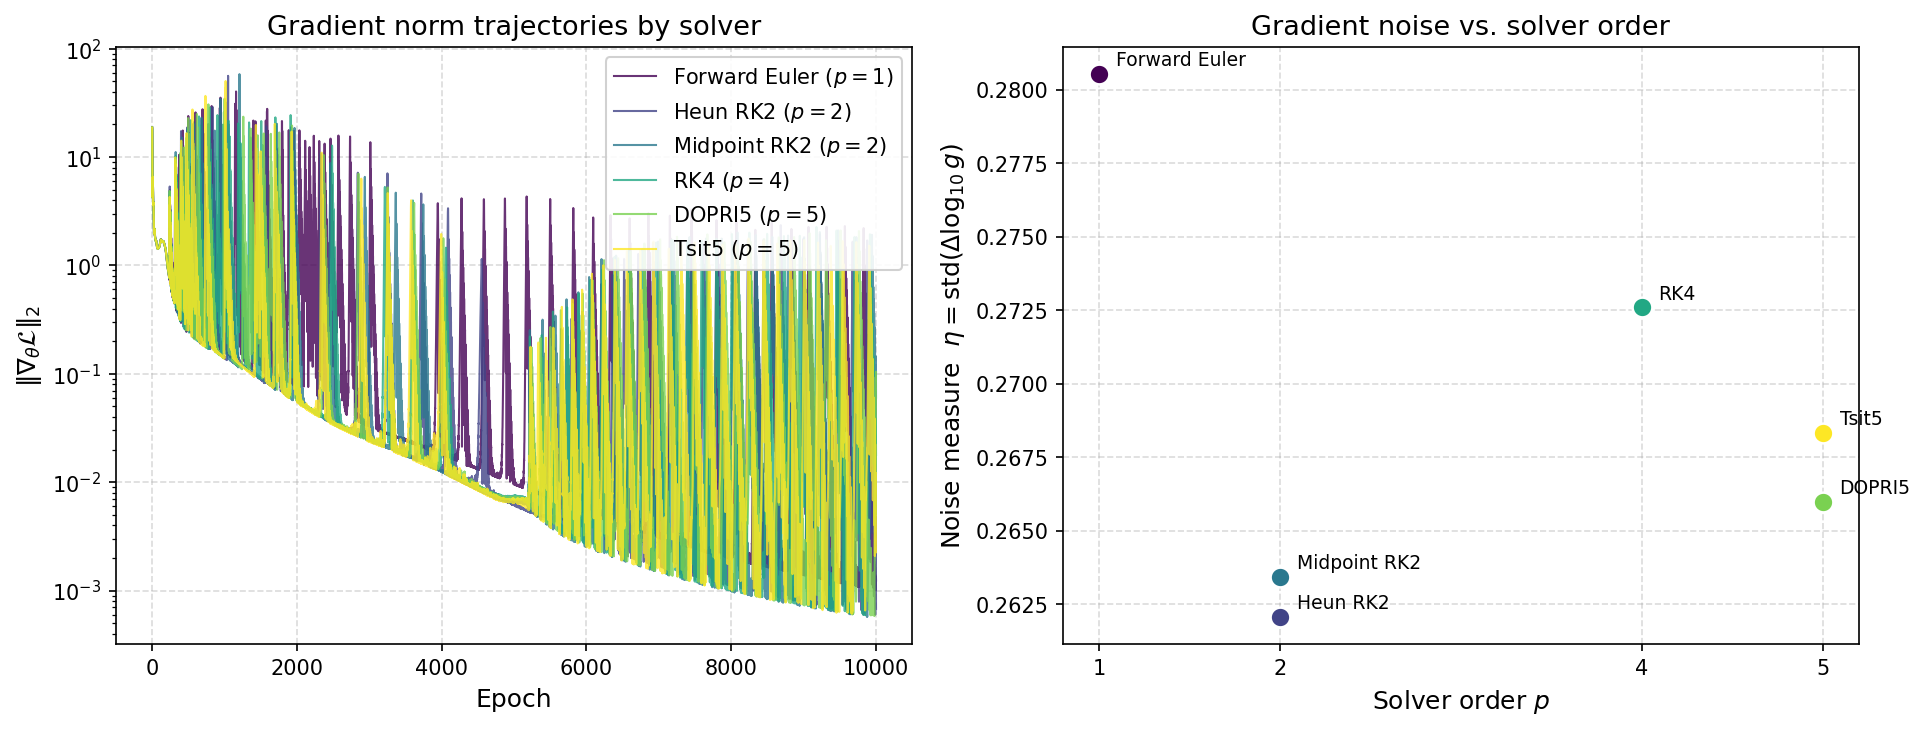
\includegraphics[width=0.85\linewidth]{figures/track_b/gradient_noise_by_order.png}
\caption{Left: gradient-norm traces, all six solvers: large sustained spike
bursts (one to two orders of magnitude above the local median) dominate every
trace, including Tsit5, independent of solver order. Right: the noise measure
$\eta$ (Equation~\ref{eq:noise-measure}) against solver order, showing the
non-monotone ranking of Table~\ref{tab:gradient-noise}.}
\label{fig:gradient-noise}
\end{figure}

\paragraph{Finding.} Gradient-norm roughness does not explain Euler's
convergence floor (Table~\ref{tab:gradient-noise}). All six traces are
instead dominated (Figure~\ref{fig:gradient-noise}) by shared,
order-independent spike bursts (a spike epoch being one whose gradient norm
exceeds $8\times$ its median over epochs 6000--10{,}000; 1176 spike epochs for
Euler and 866 for Tsit5 in the last 4000 epochs, with near-identical burst
structure). Four checks rule out a numerical defect: zero non-finite
gradients or losses across 60{,}000 logged epochs; every solver's loss falls
from $4.83$ to below $1.4\times10^{-4}$, reaching its minimum in the last 12
epochs; the loss is lower five epochs after a spike in $62$--$65\%$ of cases
($64.0\%$ pooled over all six solvers); and the median loss \emph{is} elevated
on spike epochs in every solver ($1.5$--$2.2\times$; for Tsit5,
$3.90\times10^{-4}$ against $1.80\times10^{-4}$ on calm epochs), ruling out a
spurious-gradient/still-loss signature. The most plausible reading is
edge-of-stability optimizer behaviour. Gradient descent with a fixed step size
has been observed to settle into a regime where it repeatedly overshoots the
walls of a narrowing loss valley as training approaches a sharp minimum
\cite{cohen2021eos}, and adaptive methods show a similar regime
\cite{cohen2022adaptive}. Adam at a constant learning rate
($2\times10^{-3}$, no schedule), as used here, plausibly behaves the same way,
producing this pattern of a large transient spike followed by fast recovery
rather than either smooth convergence or a genuine divergence. Because this behavior
appears with near-identical structure in Euler's and Tsit5's traces alike,
it is a property of the optimizer and the loss surface's local geometry, not
of the integrator's truncation error. Euler's convergence floor is better
explained by the earlier systematic-bias hypothesis (Section~\ref{sec:phase2}):
a first-order integrator's $O(h)$ global error biases \emph{where} the
optimizer settles, without making the path it takes to get there measurably
rougher.

\FloatBarrier
